\documentclass[10pt,notes]{beamer}
\usetheme{Madrid}
\usepackage[utf8]{inputenc}
\usepackage{amsmath}
\usepackage{amsfonts}
\usepackage{amssymb}
\usepackage{graphicx}

\usepackage{pgfpages}
\usepackage{ragged2e}

\author[PM]{Pietro Mascolo}
\title[Predicting the future]{Predicting future states using Markov Chains}
%\setbeamercovered{transparent} 
%\setbeamertemplate{navigation symbols}{} 
%\logo{} 
\institute[Optum]{\textbf{\Large{Optum Ireland Ltd.}}} 
\date{\small{April 22, 2018}}

\definecolor{optum-orange}{RGB}{232, 119, 34}
\definecolor{optum-green}{RGB}{7,133,118}
\definecolor{optum-yellow}{RGB}{234,170,0}
\definecolor{optum-gray}{RGB}{136,139,141}
\definecolor{optum-link-blue}{RGB}{0,102,204}

\mode<presentation>
 {
 \setbeamercolor*{palette primary}{use=structure,fg=white,bg=optum-orange}
 \setbeamercolor*{palette secondary}{use=structure,fg=white,bg=optum-gray}
 \setbeamercolor*{palette tertiary}{use=structure,fg=white,bg=optum-yellow}
 \setbeamercolor*{block title}{use=structure,fg=white,bg=optum-green}
 }
 
%\setbeameroption{show notes on second screen=right}


%\subject{} 
\begin{document}

	\begin{frame}
		\titlepage
	\end{frame}

%\begin{frame}
%\tableofcontents
%\end{frame}

	\section{Introduction}

	\begin{frame}{Who I am}
		\begin{columns}
			\column{0.5\textwidth}
			\begin{itemize}
   				\item Physicist;
   				\item Data Scientist;
   				\item \textbf{Python enthusiast};
   				\item \textbf{Kotlin}/Scala practitioner;
   				\item \textbf{Golang} padawan;
   				\item Ham Radio Operator (EI/IZ4VVE);
   				\item Hiker;
   				\item Karateka;
   				\item Amateur Photographer;
   				\item ...
			\end{itemize}
   			
   			\column{0.5\textwidth}
   			\begin{center}
   				
\includegraphics[width=0.8\textwidth]{imgs/me.png}
			\end{center}

		\end{columns}
	\end{frame}
	
	
	\begin{frame}{Optum - Our mission}
		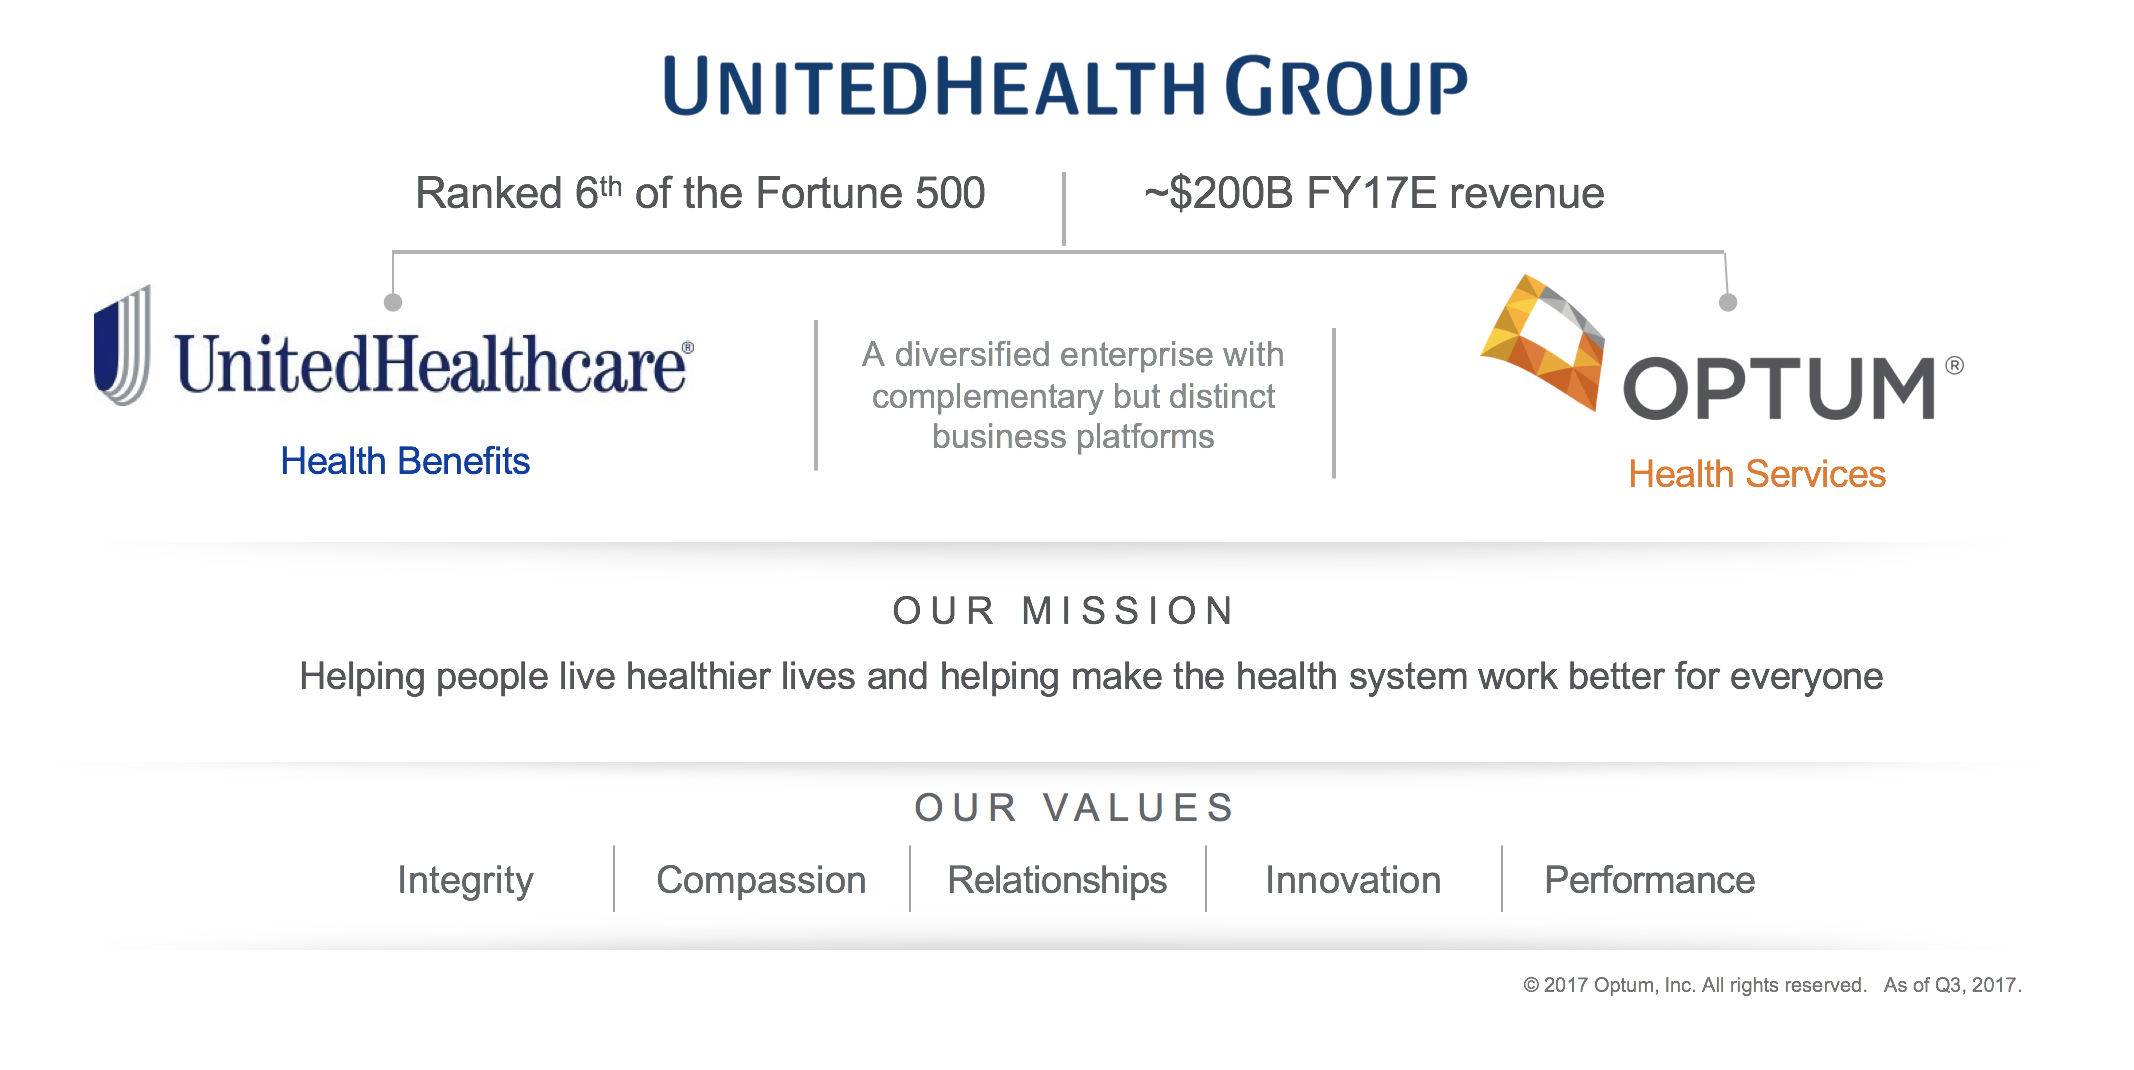
\includegraphics[width=\textwidth]{imgs/optum-mission.png}
		\note{6th in Fortune500, 270K employees as of 2018, 200B USD revenue}
	\end{frame}
	
	
	\section{Markov chains}
	\begin{frame}
	\begin{block}{Definition}
	A Markov chain is "a stochastic model describing a sequence of possible events in which the probability of each event depends only on the state attained in the previous event."[1]
\end{block}
\end{frame}
	\subsection{Definition}
	
	\subsection{Maths}
	
	\subsection{What can be done with MC}
	
	\section{Code and live demo}

\end{document}